\documentclass[12pt,a4paper]{article}
\usepackage{fontspec}
\setmainfont{Times New Roman}
\usepackage{indentfirst}
\usepackage{hyperref}
\usepackage{tikz}
\usepackage[left=2.64cm,right=2.54cm,top=2cm,bottom=2cm]{geometry}
\usepackage{geometry}
\usepackage{array}
\usepackage{color}
\usepackage{wallpaper}
\setcounter{page}{2}
\makeatletter
\definecolor{dkgreen}{rgb}{0,0.6,0}
\definecolor{gray}{rgb}{0.5,0.5,0.5}
\definecolor{mauve}{rgb}{0.58,0,0.82}
\usepackage{listings}
\pagenumbering{arabic}
\usepackage{fancyhdr}
\usepackage{lastpage}
\usepackage{minitoc}
\pagestyle{fancy}
\fancyhf{}
\rhead{21127511 Nguyễn Quốc Huy}
\lhead{INTRODUCTION TO PROGRAMING}
\rfoot{Page \thepage \hspace{1pt} of \pageref{LastPage}}
\usepackage{multicol}
\setlength{\columnsep}{1cm}
\begin{document}
\thispagestyle{empty}
\begin{LARGE}
    \begin{center}{\underline{\color{red}{\bf NATIONAL UNIVERSITY OF HO CHI MINH CITY}}}
    \end{center}
\end{LARGE}
\vspace*{1cm}
\begin{center}{\Huge \color{green}\textbf{TICTACTOE PROJECT REPORT}}
\end{center}
\ThisCenterWallPaper{1}{New_KHTN.jpg}
\vspace*{15cm}
\begin{center}{\Huge \color{cyan}\textbf{21CLC02 - Nguyễn Quốc Huy - 21127511}}
\end{center}
\vspace*{1cm}
\begin{center}
    {\Huge \color{cyan}\textbf{{INTRODUCTION TO PROGRAMING}}}
\end{center}
\newpage
\let\cleardoublepage\clearpage
\section{\textbf{\color{red}ABSTRACT}}
\begin{itemize}
    \item This Document include the report of Project - Tictactoe Game .
    \item This Project 2 has completed as version Expert.
    \item Special library is windows.h and \#pragma comment(lib, "winmm.lib") for adding music.
    \item Windows OS for running
    \item Use Super\_Mario.wav for music.
\end{itemize}
\tableofcontents

\newpage
\section{\textbf{\color{red}CHAPTER 1: GAME TUTORIAL}}
The tutorial of the tictactoe game:
\begin{itemize}
    \item  Firstly, there will be the beginning introduction ask you to play game or quit, if choose press spacebar button.
    \item  Then you wil go to the Menu select with 3 option: Tutorial, Play Game and Quit. Choose tutorial will lead you to the guidance of the game, choose playgame to continue, choose quit to end the game.
    \item  You choose to play sound during the game or not.
    \item  You can choose between playing with person (PVP) or enrivonment (PVE).
    \item  Input your name and your opponent's name.
    \item  Input size of tictactoe board (N*N) (up to you).
    \item  Input the winning check that you want, but it must be less or equal than the size.
    \item  SPECIALLY, you can input the restricted time for each player to make the game harder.
    \item  Input your icon and opponient's icon to the game.
    \item  Choose the text and background color for your game. Done, and you can enjoy the game.
    \item  The goal of this game is to achieve highest streak in one horizontal line or vertical line or diagonal line which equal than the winning check point.
    \item  Player 1 will go first.
    \item  The time restricted will countdown each move.
    \item  During the game there will be some hints for each player.
    \item  The first player get the right winning check will be the winner , do not enter the chosen coordinate.
    \item  If player insert wrong coordinate, the system will ask to insert again.
    \item  If the board is filled and none player win , there will be count as a draw match.
    \item  The statistic will be print after each match.
    \item  Finally, you can choose to play again as you want. If choose to play again, the system will save the previous statistic.
\end{itemize}
Here is the specific tutorial in the game:\\
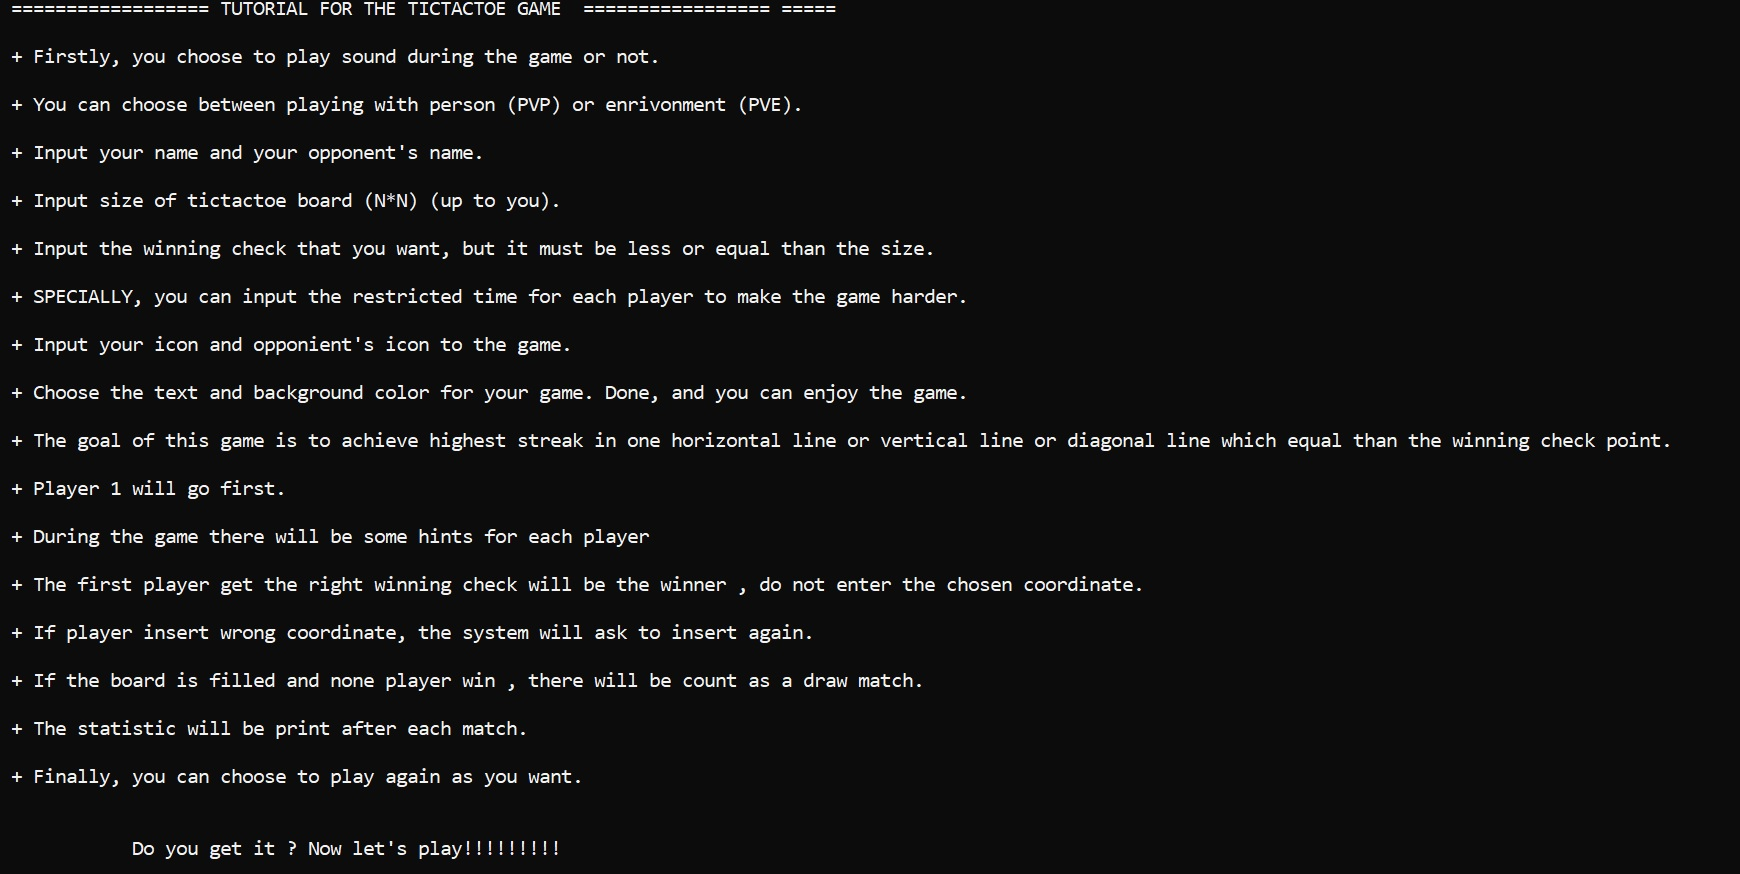
\includegraphics[scale=0.7]{picture/Tutorial.jpg}
Other pictures :\\
The beginning introduction:\\
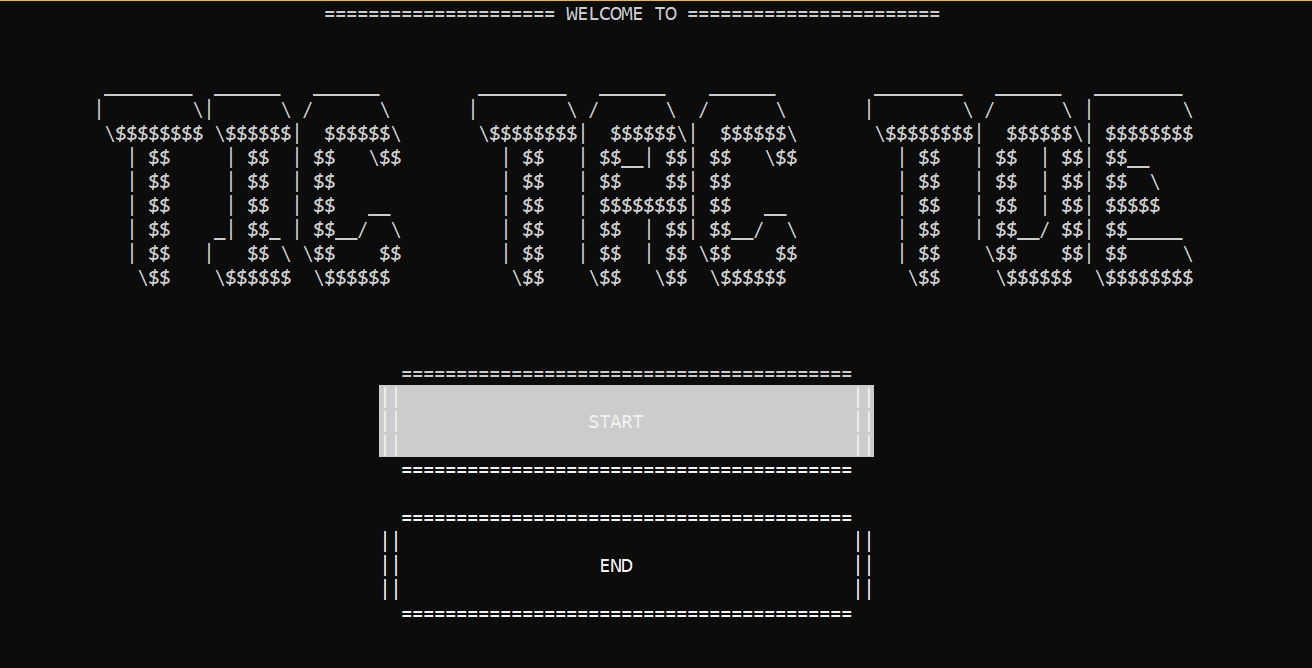
\includegraphics[scale=0.7]{picture/Intro1.jpg}\\
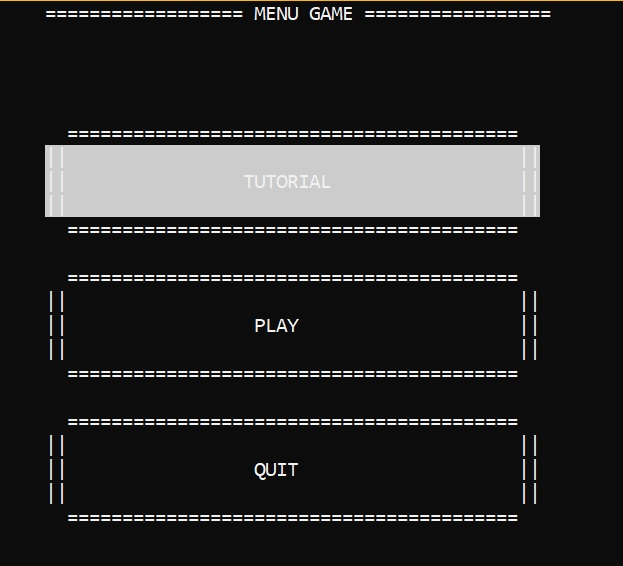
\includegraphics[scale=0.7]{picture/Intro2.jpg}\\
Choose turn on music: \\
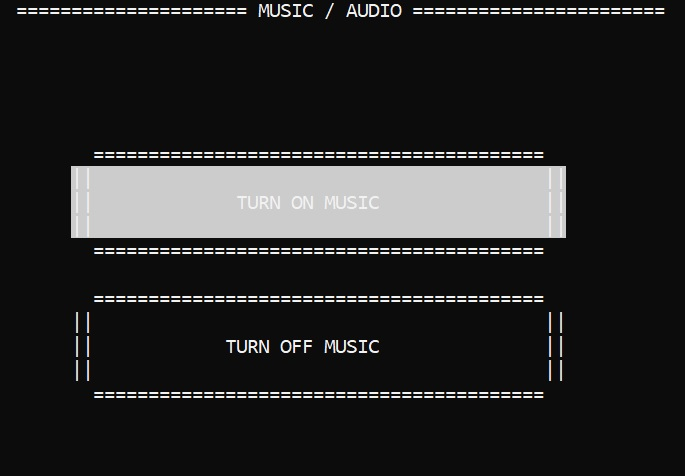
\includegraphics[scale=0.7]{picture/Music.jpg}\\
Choose mode (PVP or PVE): \\
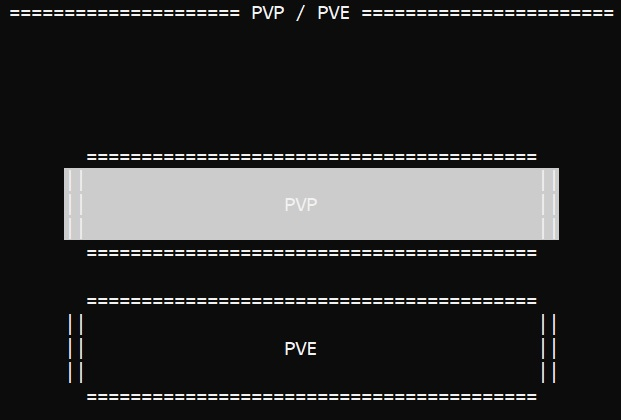
\includegraphics[scale=0.7]{picture/PVP_PVE.jpg}\\
Setting display: \\
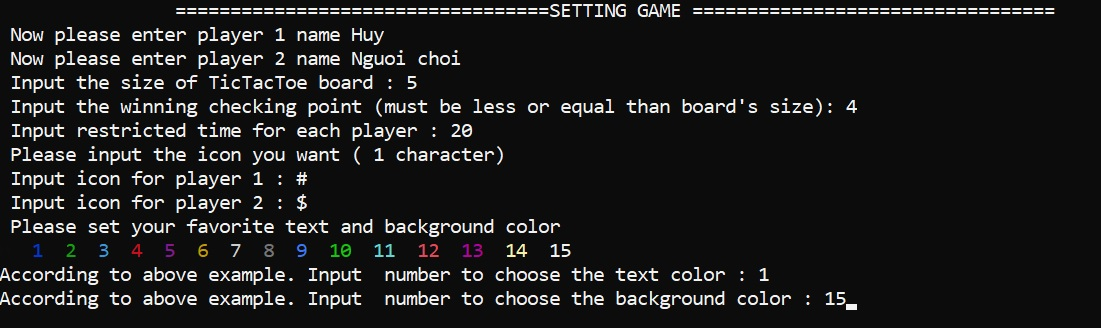
\includegraphics[scale=0.7]{picture/Setting_Display.jpg}\\ \\ \\ \\
During playing the game display: \\ 
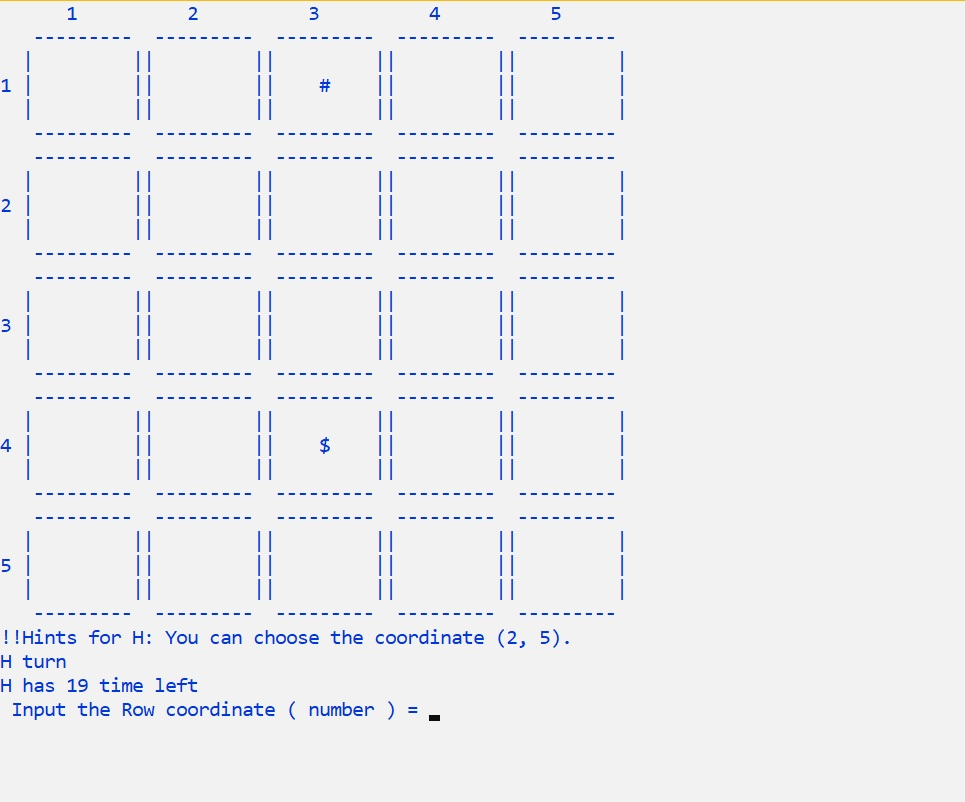
\includegraphics[scale=0.7]{picture/Playing.jpg}\\ \\ \\
Winning and statistic display: \\
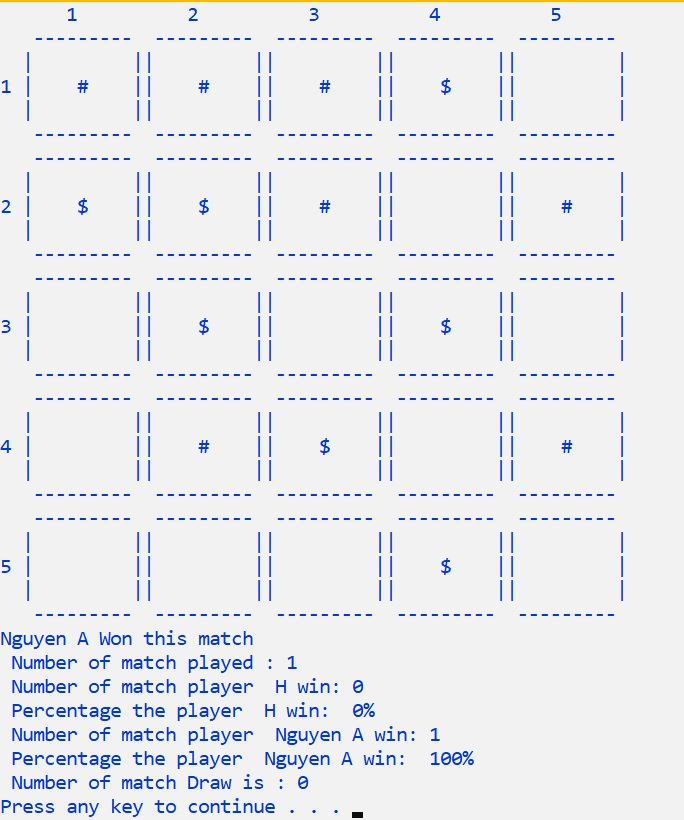
\includegraphics[scale=0.7]{picture/Winning.jpg}\\ \\ \\ \\ \\ \\ \\
Ending option: \\
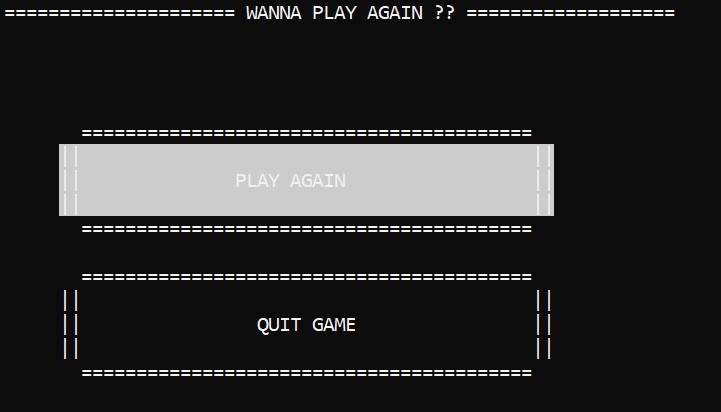
\includegraphics[scale=0.7]{picture/PlayAgain.jpg}\\
\section{\textbf{\color{red}CHAPTER 2: SOURCE CODE DESCRIPTION}}
\Large \subsection{\color{blue}\textbf{STRUCTURES FOR TICTACTOE GAME} }
Including 4 structures:
\begin{itemize}
    \item Point : include horizontal and verrtical point for a board.
    \item Suggestion : include row and collumn need for Suggesting Functions.
    \item Information : include main informations for each player such as: playername, icon, winning, Point Coordinate,...
    \item Tictactoe : include the main informations nead for the board such as: size, Backgroundcolor, Textcolor, wincheck, countdraw, Information player,....
\end{itemize}
\Large \subsection{\color{blue}\textbf{PRINT BOARD FUNCTIONS} }
The Print Board Functions include:
\begin{itemize}
    \item Print\_horizontal\_coordinates : to print the exactly coordinate in each col.
    \item Print\_horizontal\_line : to print the completely board.
    \item Print\_vertical\_line : to print the completely board.
    \item Print\_Board : combine with 3 above functions to print a completely board with the coordinate and what player move.
\end{itemize}
\Large \subsection{\color{blue}\textbf{RANDOM FUNCTIONS FOR PVE} }
The Random Functions are used for setting PVE mode that playing automatically:
\begin{itemize}
    \item random\_PVE : to give a randomly number in range.
\end{itemize}
\Large \subsection{\color{blue}\textbf{SUGGESTING FUCTIONS} }
The Suggesting Functions are used for help player to move when they need :
\begin{itemize}
    \item SuggestionPlayer1 : to give a randomly coordinate different from the chosen box for player 1 to play.
    \item SuggestionPlayer2 : to give a randomly coordinate different from the chosen box for player 2 to play.
\end{itemize}
\Large \subsection{\color{blue}\textbf{INPUT FUCTIONS} }
 The Input Functions are used for complete all information need in the game by the input of player :
\begin{itemize}
     \item Init\_Playername : use for input the name of both player.
     \item Init\_PVE\_Playername : automatically set the name for the bot player.
     \item Init\_Restricted\_Time : use for input the restricted time for both player.
     \item Init\_Board : use for set the board clear, empty to start the game.
     \item Input\_XPlayer\_Turn : use for player 1 to input the coordinates of his/her move and also check if it is a valid move or not.
     \item Input\_Environment\_Player\_Turn : use for player bot automatically set its coordinates that does not similar to the other previous moves.
     \item Input\_OPlayer\_Turn : use for player 2 to input the coordinates of his/her move and also check if it is a valid move or not.
     \item BackgroundColor : use to set the text and the background color of the match.
     \item Setting\_Color : combine with the BackgroundColor fuction and let the player input to set the color. 
\end{itemize}
\Large \subsection{\color{blue}\textbf{CHECK WIN FUCTIONS} }
 The Check win Functions are used for make sure the player can win with the right check win point and also check draw :
\begin{itemize}
     \item Check\_Horizontal\_Winner : use for checking if there are any consecutive characters in a horizontal line or not.
     \item Check\_Vertical\_Winner : use for checking if there are any consecutive characters in a verrtical line or not.
     \item Check\_Diagonal\_Winner : use for checking if there are any consecutive characters in a diagonal line or not.
     \item Check\_Vice\_Diagonal\_Winner : use for checking if there are any consecutive characters in a vice diagonal line or not.
     \item Check\_Above\_Diagonal\_Winner : use for checking if there are any consecutive characters in a above diagonal line or not.
     \item Check\_Below\_Diagonal\_Winner : use for checking if there are any consecutive characters in a below diagonal line or not.
     \item Check\_Above\_Vice\_Diagonal\_Winner : use for checking if there are any consecutive characters in a above vice diagonal line or not.
     \item Check\_Below\_Vice\_Diagonal\_Winner : use for checking if there are any consecutive characters in a below vice diagonal line or not.
     \item Check\_Winner : combine with above functions to make the completely check win function that true with all case of N*N board.
     \item Draw\_Game : use for check if the board has no move space to move or not and will draw if there isn't any space else.
\end{itemize}
\Large \subsection{\color{blue}\textbf{RESULT FUCTIONS} }
The Result Functions are used for combine all the functions above to a clear function that contain everything need for the game:
\begin{itemize}
    \item PlayGame : include the input functions, print board functions, check win functions,.... and combine them into a make sense match.
    \item Count\_Statistic : output all the information when match end: win percentage, draw percentage, who win the most, match played,...
\end{itemize}
\Large \subsection{\color{blue}\textbf{TUTORIAL FUCTION} }
\begin{itemize}
    \item Tutorial : show specificly all the guidances for the game.
\end{itemize}
\Large \subsection{\color{blue}\textbf{OTHER GAME'S INTRO FUCTIONS} }
\begin{itemize}
    \item gotoxy : to move the cursor to the exactly coordinate.
    \item INTRO and INTRO\_NEXT : To show the beginning of the game including menu, options,...
    \item ENDING : To ask if the player want to play again or not.
    \item Music : To ask the player want to play music or not.
    \item PVE : To ask which option player choose between PVP and PVE mode.
    \item Init\_Setting : Include some functions in INPUT FUNCTIONS and require player to input information.
\end{itemize}
\section{\textbf{\color{red}REFERENCES}}
This Tictactoe game was completed thanks to the supporting from:
\begin{itemize}
    \item Starting Out with C++ from Control Structures to Objects 8th Edition by TONY GADDIS
    \item The suggestion from Mr. Thong and Mrs. Nhi.
    \item The ideas from the code of Mr. Thong each pratical class.
    \item Gotoxy supporting :\url{https://www.youtube.com/watch?v=fOW0Fgqx3XU} for the gotoxy function in the game.
    \item Music setting : \url{https://daynhauhoc.com/t/long-nhac-mp3-vao-ung-dung-console-c/34035} for adding music into the game.
\end{itemize}


\end{document}